\documentclass[aspectratio=169,12pt]{beamer}
\usetheme{default}
\setbeamertemplate{navigation symbols}{}
\setbeamertemplate{footline}[frame number]
\setbeamertemplate{itemize items}[circle]
\setbeamerfont{frametitle}{size=\Large,series=\bfseries}
\setbeamercolor{frametitle}{fg=black}
\setbeamercolor{structure}{fg=black!75}
\usepackage{amsmath,amssymb,booktabs,graphicx,tikz,catchfile}
\usetikzlibrary{arrows.meta,positioning}
\newcommand{\dir}{claude-filter-explainer-11.12.26-files}
\input{\dir/numbers.tex}   % written by claude-filter-explainer-11.12.26-figures.R
\input{\dir/numbers-fullgrid.tex}   % written by claude-filter-explainer-11.12.26-fullgrid.R
\CatchFileDef{\rowsfullgrid}{\dir/rows-fullgrid.tex}{}
\CatchFileDef{\rowsfullgridcompare}{\dir/rows-fullgrid-compare.tex}{}
\newcommand{\N}{\mathcal{N}}
\newcommand{\muted}[1]{{\color{black!55}#1}}
\definecolor{fc}{HTML}{EB6834}
\definecolor{an}{HTML}{2A78D6}

\title{The OR joint-update filter}
\subtitle{tracking carbon, disturbances and process error together}
\author{Claude}
\date{November 12, 2026}

\begin{document}

\begin{frame}
  \titlepage
\end{frame}

%---------------------------------------------------------------------------
\begin{frame}{What the filter estimates}
  Each year $t$, at one site, from observations of wood carbon $y_t$:
  \medskip
  \begin{itemize}
    \item the carbon state $x_t = (\text{leaf},\ \text{soil},\ \text{wood})$
    \item whether a disturbance happened, and which kind: $z_t \in \{0, 1, \dots, K\}$
    \item how large the model's process error is: precision $\tau$
  \end{itemize}
  \bigskip
  All three are uncertain and depend on each other, so they are updated jointly:
  \begin{itemize}
    \item a big drop in $y_t$ is either a disturbance or a large process error,
    \item and the process error decides how far a forecast can move without a disturbance.
  \end{itemize}
\end{frame}

%---------------------------------------------------------------------------
\begin{frame}{Model: one year}
  \[
    x_t \;=\;
    \begin{cases}
      f(x_{t-1}) + e_t & z_t = 0 \quad\text{(undisturbed)}\\[3pt]
      d_k\big(f(x_{t-1}) + e_t\big) & z_t = k \quad\text{(disturbance type } k\text{)}
    \end{cases}
    \qquad
    y_t = x_{t,\text{wood}} + \varepsilon_t
  \]
  \begin{itemize}
    \item $f$: one year of the VSEM forest model, driven by that year's light (PAR)
    \item $e_t \sim \N(0, Q)$, \quad $Q = \operatorname{diag}\big(\sigma^2_\text{leaf},\ \sigma^2_\text{soil},\ 1/\tau\big)$
      \quad \muted{(leaf, soil: calibrated; wood: learned)}
    \item $\varepsilon_t \sim \N(0, R_t)$, \quad $R_t = a\,y_t + b$ \quad \muted{(error grows with biomass)}
    \item $P(z_t = k) = \beta_{t,k}$: background disturbance rates, or the disturbance
          product's accuracy in the years it flags a disturbance
  \end{itemize}
\end{frame}

%---------------------------------------------------------------------------
\begin{frame}{Model: disturbances and their process error}
  Disturbance $k$ keeps a random \emph{fraction} of leaf and wood; part of the removed
  carbon goes to the soil:
  \[
    \text{leaf}', \text{wood}' \sim \N\!\big(\mu_{0,k}\cdot\text{old},\ V_{0,k}\cdot\text{old}^2\big),
    \qquad
    \text{soil}' = \text{soil} + \alpha\,(\text{removed})
  \]
  \muted{$K = 16$ types: other, cut, fire, biotic, each split into size clusters fitted to observed biomass losses.}
  \bigskip

  The year's process error happens before the disturbance, so it is scaled by the
  same fraction:
  \[
    \operatorname{Var}(\text{process error} \mid z_t = k) \;=\; D_k\, Q\, D_k,
    \qquad D_k = \operatorname{diag}\big(\mu_{0,k}^\text{leaf},\ 1,\ \mu_{0,k}^\text{wood}\big)
  \]
  \muted{Leaf and wood keep $\mu_0^2$ of their process variance; the soil keeps all of it.}
\end{frame}

%---------------------------------------------------------------------------
\begin{frame}{The posterior the filter carries}
  For every value $\tau_g$ on a grid ($g = 1..200$, log-spaced, process sd $0.01$--$3$):
  \[
    p(x_t \mid \tau_g, y_{1:t}) \;\approx\; \sum_{j} w_{g,j}\; \N(x_t;\ m_{g,j},\ C_{g,j})
    \qquad j \in \{\text{undisturbed},\ \text{disturbed}\}
  \]
  and a weight for each grid point:
  \[
    \pi_t(g) \;=\; P(\tau = \tau_g \mid y_{1:t})
  \]
  \medskip
  So the full posterior is a mixture of $2 \times 200$ Gaussians.
  Every summary (state, disturbance, $\tau$) averages over it.
\end{frame}

%---------------------------------------------------------------------------
\begin{frame}{One assimilation step}
  \centering
  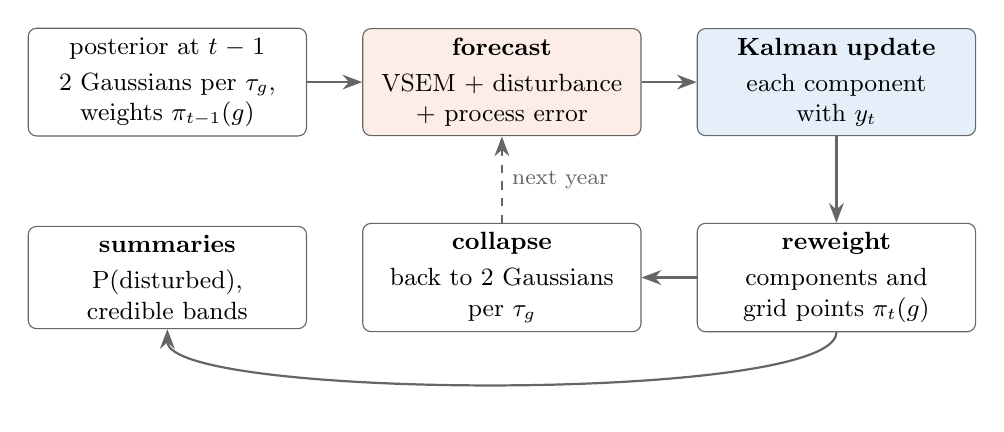
\begin{tikzpicture}[
      box/.style={draw=black!60, rounded corners=3pt, align=center, minimum height=1.25cm, text width=3.3cm, font=\small},
      arr/.style={-{Stealth[length=2.5mm]}, thick, black!60}]
    \node[box] (prev) {posterior at $t-1$\\[2pt] $2$ Gaussians per $\tau_g$,\\ weights $\pi_{t-1}(g)$};
    \node[box, right=0.7cm of prev, fill=fc!12] (fc) {\textbf{forecast}\\[2pt] VSEM + disturbance\\ + process error};
    \node[box, right=0.7cm of fc, fill=an!12] (ku) {\textbf{Kalman update}\\[2pt] each component\\ with $y_t$};
    \node[box, below=1.1cm of ku] (tau) {\textbf{reweight}\\[2pt] components and\\ grid points $\pi_t(g)$};
    \node[box, left=0.7cm of tau] (col) {\textbf{collapse}\\[2pt] back to 2 Gaussians\\ per $\tau_g$};
    \node[box, left=0.7cm of col] (sum) {\textbf{summaries}\\[2pt] P(disturbed),\\ credible bands};
    \draw[arr] (prev) -- (fc);
    \draw[arr] (fc) -- (ku);
    \draw[arr] (ku) -- (tau);
    \draw[arr] (tau) -- (col);
    \draw[arr] (tau.south) .. controls +(0,-0.9) and +(0,-0.9) .. (sum.south);
    \draw[arr, dashed] (col.north) -- node[right, font=\footnotesize] {next year} (col.north |- prev.south);
  \end{tikzpicture}
  \bigskip

  {\small Each grid point $\tau_g$ runs its own small mixture filter; they share the forecast simulations.}
\end{frame}

%---------------------------------------------------------------------------
\begin{frame}{Forecast: push the posterior through VSEM}
  VSEM is nonlinear, so the forecast moments are estimated by \textbf{importance sampling}:
  \begin{enumerate}
    \item draw $N = 100$ states $x^{(n)}$ from the whole previous mixture (all $g$, $j$)
    \item run each through one year of VSEM: $f(x^{(n)})$ \muted{(the expensive part: done once)}
    \item for each component $(g,j)$, weight the samples by how likely it made them:
      \[
        W_{g,j}^{(n)} \;\propto\; \frac{\N\big(x^{(n)};\ m_{g,j}, C_{g,j}\big)}{q\big(x^{(n)}\big)}
        \qquad q = \text{the mixture the samples came from}
      \]
    \item for each disturbance type $k$: apply $d_k$ to the simulated states, take the weighted
          mean and covariance, and add the process error ($Q$ or $D_kQD_k$, with $1/\tau_g$ for wood)
  \end{enumerate}
  \medskip
  Result: forecast components $(g, j, k)$ with means $\hat m$, covariances $\hat C$ and
  prior weights $w_{g,j}\,\beta_{t,k}$.
\end{frame}

%---------------------------------------------------------------------------
\begin{frame}{Forecast and analysis in a disturbance year}
  \centering
  \includegraphics[width=0.82\textwidth]{\dir/syn-mixture.pdf}\\
  {\small Synthetic run, year 10 (a harvest). The forecast mixture has an undisturbed mode and a
  disturbed mode near zero. The observation picks the disturbed one.}
\end{frame}

%---------------------------------------------------------------------------
\begin{frame}{Kalman update: each component separately}
  Within a forecast component the model is linear-Gaussian, so the exact update applies
  (observing wood, $H = (0, 0, 1)$):
  \[
    s = \hat C_{33} + R_t, \qquad
    K = \hat C_{\cdot 3} / s, \qquad
    m^a = \hat m + K\,(y_t - \hat m_3), \qquad
    C^a = \hat C - K\,\hat C_{3\cdot}
  \]
  \medskip
  Each component also gets the likelihood of the observation, its predictive density:
  \[
    L_{g,j,k} \;=\; \N\big(y_t;\ \hat m_3,\ s\big)
  \]
  \muted{A component that predicted $y_t$ badly keeps its update but loses its weight.}
\end{frame}

%---------------------------------------------------------------------------
\begin{frame}{Reweighting: components and the process-error grid}
  Components, within each grid point (Bayes' rule over $j, k$):
  \[
    w^a_{g,j,k} \;\propto\; w_{g,j}\,\beta_{t,k}\; L_{g,j,k}
  \]
  Grid points: each one's evidence is how well its whole forecast predicted $y_t$:
  \[
    \pi_t(g) \;\propto\; \pi_{t-1}(g)\; \underbrace{\sum_{j,k} w_{g,j}\,\beta_{t,k}\,L_{g,j,k}}_{p(y_t \mid \tau_g,\ y_{1:t-1})}
  \]
  \begin{itemize}
    \item $\pi_0(g)$: prior mass of the grid cell around $\tau_g$
    \item small $\tau$ (large process error) explains jumps but spreads its forecast thin;
          large $\tau$ forecasts sharply but is penalized when the data move
  \end{itemize}
\end{frame}

%---------------------------------------------------------------------------
\begin{frame}{Collapse: keep the mixture from growing}
  After the update each grid point has $2 \times (K+1) = 34$ components; left alone, the
  count would multiply every year. So, per grid point, the components are merged into two:
  \begin{itemize}
    \item \textbf{undisturbed this year} ($k = 0$), and \textbf{disturbed this year} ($k \ge 1$)
  \end{itemize}
  each replaced by one Gaussian with the same weight, mean and covariance:
  \[
    w = \sum_i w^a_i, \qquad
    m = \sum_i \tfrac{w^a_i}{w}\, m^a_i, \qquad
    C = \sum_i \tfrac{w^a_i}{w} \big(C^a_i + m^a_i m^{a\top}_i\big) - m\,m^\top
  \]
  \muted{This is the best single Gaussian (in KL divergence) for each group. Keeping the disturbed
  group separate lets next year's forecast still carry a post-disturbance branch.}
\end{frame}

%---------------------------------------------------------------------------
\begin{frame}{Summaries}
  Everything averages over the grid and the components, with weights $\pi_t(g)\,w^a_{g,j,k}$:
  \[
    P(\text{disturbed in year } t \mid y_{1:t}) \;=\; \sum_g \pi_t(g) \sum_{j}\sum_{k \ge 1} w^a_{g,j,k}
  \]
  \[
    P(x_{t,\text{wood}} \le u \mid y_{1:t}) \;=\; \sum_{g,j,k} \pi_t(g)\, w^a_{g,j,k}\;
      \Phi\!\Big(\tfrac{u - m^a_3}{\sqrt{C^a_{33}}}\Big)
  \]
  \begin{itemize}
    \item 95\% credible band: solve for $u$ at $0.025$ and $0.975$ (root-finding on the mixture CDF)
          \muted{(can be skewed or bimodal, unlike mean $\pm$ 2 sd)}
    \item process error: $\pi_t(g)$ is the posterior of $\tau$; reported as
          $\sqrt{\mathbb{E}[1/\tau \mid y_{1:t}]}$ or quantiles of $1/\sqrt{\tau}$
    \item one-step-ahead forecast of $y_t$: the same mixture before the update; its PIT
          checks calibration
  \end{itemize}
\end{frame}

%---------------------------------------------------------------------------
\begin{frame}{Synthetic test: set-up}
  The multi-pool version of the filter on simulated data with a known truth:
  \begin{itemize}
    \item one site, 25 years, a harvest in year 10 (keeps $\sim$10\% of leaf and wood)
    \item every pool observed, $R = \operatorname{diag}(0.25, 10, 1)$
    \item true process sd $0.32$ for every pool, unknown to the filter: all three
          precisions are learned, on a $16^3$ grid
    \item prior $P(\text{disturbed}) = 0.05$ every year
    \item 21 random seeds: new drivers, parameters, truth and observations each time
  \end{itemize}
  \medskip
  \muted{Differences from the OR model: there only wood is observed and only the wood $\tau$ is learned (200-point grid).}
\end{frame}

%---------------------------------------------------------------------------
\begin{frame}{Synthetic: states and disturbance (seed 42)}
  \centering
  \includegraphics[width=\textwidth]{\dir/syn-states.pdf}
\end{frame}

%---------------------------------------------------------------------------
\begin{frame}{Synthetic: learning the process error (seed 42)}
  \centering
  \includegraphics[width=\textwidth]{\dir/syn-tau.pdf}\\[4pt]
  {\small The posterior moves off the log-uniform prior but stays wide after 25 annual
  observations: the 95\% band spans about a factor of 10 and covers the truth, with the
  median below it and $\sqrt{\mathbb{E}[1/\tau]}$ above it.}
\end{frame}

%---------------------------------------------------------------------------
\begin{frame}{Synthetic: 21 seeds}
  \centering
  \includegraphics[width=0.72\textwidth]{\dir/syn-seeds.pdf}\\[-2pt]
  \begin{itemize}\footnotesize
    \item detection: $P(\text{disturbed})$ in year 10 has median \SynDetMed{} (min \SynDetMin);
          above 0.5 in \SynDetN{} of 21 seeds
    \item false alarms ($P > 0.5$ in other years): \SynFAN{} of \SynYears{} seed-years (\SynFASeeds{} seeds)
    \item truth inside the 95\% band: \SynCov{} of years
    \item RMSE of the median relative to the filter given the true $\tau$: \SynRMSE{} (medians)
    \item process sd at year 25: truth inside the 95\% band in \SynSDCov{} of 21 seeds;
          posterior median / truth \SynSDMed{} (medians)
  \end{itemize}
\end{frame}

%---------------------------------------------------------------------------
\begin{frame}{OR test run: site 300}
  \centering
  \includegraphics[width=0.8\textwidth]{\dir/or-site300.pdf}\\[2pt]
  {\footnotesize GEDI heteroskedastic $R$, bias correction, gamma prior on $\tau$. Wood falls from 15 to 5 kg C m$^{-2}$
  over 2003--04: $P(\text{disturbed}) = 1$ in both years, with or without the product. The first forecast comes
  from the population-wide initial-condition prior, hence its miss in 1990.}
\end{frame}

%---------------------------------------------------------------------------
\begin{frame}{OR: 100 random sites}
  \centering
  \includegraphics[width=0.88\textwidth]{\dir/or-100.pdf}\\[2pt]
  {\footnotesize Left: PIT of each observation after the first under its one-step-ahead forecast.
  Too many land mid-range (\ORPitIn{} in the central 95\%, \ORPitMid{} in the central 50\%):
  the forecasts are too wide. Right: without the product, every site with a one-year
  loss above 3 kg C m$^{-2}$ is detected (\ORDetBig), none with a loss below 1 (\ORDetSmall).
  Most sampled sites are product-flagged: the sites were drawn stratified by disturbance class.}
\end{frame}

%---------------------------------------------------------------------------
\begin{frame}{OR full grid: set-up and metrics}
  All 538 sites $\times$ 4 observation-error models $\times$ with / without the disturbance product
  = \FGRuns{} runs, with the defaults: bias correction on, process error propagated through
  the disturbance, gamma prior on $\tau$. \muted{About 15 minutes on 8 cores.}
  \medskip
  \begin{itemize}\small
    \item \textbf{PIT in 95\% / 50\%}: share of observations inside the central 95\% / 50\% of their
          one-step-ahead forecast \muted{(calibrated: 95\% / 50\%)}
    \item \textbf{final in band}: last observation inside the 95\% analysis band
    \item \textbf{detect, loss $>$ 3}: $P(\text{disturbed}) > 0.5$ in years where observed wood fell
          by more than 3 kg C m$^{-2}$ (\FGNBig{} site-years)
    \item \textbf{detect, flagged}: $P(\text{disturbed}) > 0.5$ in the years the product flags
    \item \textbf{false alarm}: $P(\text{disturbed}) > 0.5$ in unflagged years with $|$change$| < 0.5$ (\FGNQuiet{} site-years)
    \item \textbf{process sd}: median over sites of $\sqrt{\mathbb{E}[1/\tau \mid y]}$ in 2017 (kg C m$^{-2}$)
  \end{itemize}
\end{frame}

%---------------------------------------------------------------------------
\begin{frame}{OR full grid: results by setting}
  \centering\footnotesize\setlength{\tabcolsep}{4pt}
  \begin{tabular}{llccccccc}
    \toprule
    & & \multicolumn{2}{c}{PIT in} & final & \multicolumn{2}{c}{detect} & false & process \\
    observation error & product & 95\% & 50\% & in band & loss $>$ 3 & flagged & alarm & sd \\
    \midrule
    \rowsfullgrid
    \bottomrule
  \end{tabular}
  \smallskip
  \begin{itemize}\scriptsize
    \item Forecasts are too wide everywhere (60--90\% in the central 50\%), most with LandTrendr's larger $R$.
    \item Large losses are found without the product under GEDI errors (89--99\%); LandTrendr's larger
          $R$ hides some (60--68\%). No false alarms in quiet years.
    \item Many product-flagged years show little wood loss; under GEDI's small $R$ the data overrule the product.
  \end{itemize}
\end{frame}

%---------------------------------------------------------------------------
\begin{frame}{OR full grid: forecast calibration}
  \centering
  \includegraphics[width=\textwidth]{\dir/fullgrid-pit.pdf}\\[2pt]
  {\footnotesize PIT of every observation after the first, all 538 sites. A calibrated forecast gives a flat
  histogram (dashed). The hump means the forecasts are too wide; it is largest with LandTrendr's $R$.}
\end{frame}

%---------------------------------------------------------------------------
\begin{frame}{OR full grid: detection}
  \centering
  \includegraphics[width=\textwidth]{\dir/fullgrid-detection.pdf}\\[2pt]
  {\footnotesize Every site-year, 1991--2012, GEDI heteroskedastic $R$. Without the product, $P(\text{disturbed})$
  jumps to 1 once the loss passes about 1--2 kg C m$^{-2}$. With it, flagged years with no visible loss
  get intermediate probabilities: the prior says disturbed, the data disagree.}
\end{frame}

%---------------------------------------------------------------------------
\begin{frame}{Does propagating the process error matter?}
  Averages over the 8 settings; the earlier grid gave disturbed components no process error:
  \medskip

  \centering\footnotesize
  \begin{tabular}{lccccccc}
    \toprule
    process error & \multicolumn{2}{c}{PIT in} & final & \multicolumn{2}{c}{detect} & false & process \\
    after disturbance & 95\% & 50\% & in band & loss $>$ 3 & flagged & alarm & sd \\
    \midrule
    \rowsfullgridcompare
    \bottomrule
  \end{tabular}
  \bigskip

  \raggedright\small
  Almost no difference. The added variance, $\mu_0^2 / \tau \lesssim 0.02$, is small next to the spread
  of the disturbance size itself: $V_0 \cdot \text{old}^2$ is roughly 1--30 for a 15 kg C m$^{-2}$ stand.
\end{frame}

%---------------------------------------------------------------------------
\begin{frame}{Summary}
  \begin{itemize}
    \item The posterior is a mixture: 2 Gaussians per process-error grid point, plus a weight per grid point.
    \item Forecast: one batch of VSEM runs, reused for every component by importance weighting;
          each disturbance type and the process error are applied to it.
    \item Update: an exact Kalman update per component; the likelihoods reweight the components
          (\(\Rightarrow\) disturbance) and the grid points (\(\Rightarrow\) process error).
    \item Collapse to 2 Gaussians per grid point keeps the cost fixed over time.
    \item Summaries average over everything: $P(\text{disturbed})$, mixture-quantile credible bands,
          the posterior of the process sd.
    \item On the OR grid: large losses are detected without false alarms, but the one-step-ahead
          forecasts are too wide; propagating the process error through the disturbance changes little.
  \end{itemize}
\end{frame}

\end{document}
